\chapter{Entropy-based measures of verbal valency}\label{chapter:entropy}

While the previous chapter has demonstrated that corpus-based transitivity ratios can serve a useful basis for typological comparison, it is still is a relatively simple metric that captures but one aspect of verbal valency. Put another way, transitivity ratio is a subset of the scope needed to investigate verbal valency, as it concerns only one type of verb dependent, i.e., the object, and one feature of this dependent, i.e., its presence or absence. 

This chapter undertakes to expand the scope of investigation accordingly, to cover both more verb dependent types and more features of them. Instead of performing exhaustive comparisons on each individual feature of each dependent, the focus is instead on measuring the alternations of valency frames (diathesis alternations), i.e., range of the valency frames in which a verb appears and how often it appears with them. To that end, I propose novel metrics of verbal valency based on entropy, a concept from information theory that quantifies the average amount of information expected from a variable, and look at whether it reflects universals of how languages structure their verbal lexicons.

% In §X, valency frame entropy conditioned on the verb is calculated to measure ; §X, ablation study to see how different aspects of valency frame encoding contribute; in §X, the reverse verb entropy conditioned on the frame is calculated as a symmetric check on the measures. 

\section{Valency frame, frequency and the efficient organization of the lexicon}

Cognitive linguists and typologists have increasingly sought to integrate the two approaches in the same functionalist research paradigm \citep{croft2016}. Among others is research that seeks to examine and explain language-internal and cross-linguistic features of human languages through the lens of communicative efficiency, at various levels including the lexicon, syntax and morphology (see \citealp{gibson2019} for a survey). 

An early example where efficiency is used to explain phenomena in human languages is the work of George Kingsley \citet{zipf1935,zipf1949}. He first studied what is now known as Zipf's law, namely the empirical observation that ``the magnitude of words tends, on the whole, [stands] in an inverse (not necessarily proportionate) relationship to the number of occurrences'', and sought to explain it through the principle of least effort. This observation has been corroborated in psycholinguistic studies which show a consistent ``frequency effect'' for both open and closed class word \citep{segui1982,marslen-wilson1990}, where more frequently occurring words have a higher resting activation, making their lexical retrieval easier. 

That the most frequent lexical items are also more likely to be associated with irregularity is not surprising. This correlation between frequency and irregularity has most often been hypothesized and studied for morphology \citet{wu2019}. Already \citet{bybee1998} postulates a trade-off in the lexical memory that ``being easier to access, they are less likely to be replaced by regular formations''. The same trade-off would lead us to predict a similar relationship between the frequency of a verb and its associated morphosyntactic valency frame as well.

This is particularly true as psycholinguistic studies have also consistently shown the effect of semantic and syntactic attributes of the verb on online sentence processing \citep{shapiro1987,collina2001}. However, results differ on whether subcategorization (syntactic), thematic frames (semantic) or both have an effect on lexical processing. \citet{shapiro1987} reported that RTs for lexical decisions increased as the function of the number of thematic options instead of subcategorization options. In contrast, \citet{shetreet2007} reported on an fMRI study on Hebrew speakers, shows that the number of options in terms of subcategorization and thematic frames is better correlated to activity in the cortical areas that are associated with linguistic processing, as opposed to the number of complements or thematic frames. \todo{this section needs rework}

\section{Experiment 2: Valency frame entropy}
\subsection{Measuring valency frame entropy in UD}

Besides the information about transitivity, UD annotations make available further information that are related to the morphosyntactic encoding of valency frame, including information about further dependents, word order, as well as case and adpositional markings. In this experiment, we make use of such information for a more fine-grained characterization of the variation in valency frame encoding for different verbs using entropy-based measures.

\begin{table}
  \centering
  \begin{tabular}{ll}
    \toprule
    \textbf{UD label} & \textbf{Dependent} \\
    \midrule
    \textsc{nsubj} & nominal subject \\
    \textsc{obj} & object \\
    \textsc{csubj} & clausal subject \\
    \textsc{ccomp} & clausal complement \\
    \textsc{xcomp}   & open clausal complement \\
    \midrule
    \textsc{iobj} & indirect object \\
    \textsc{obl} & oblique nominal \\
    \textsc{expl} & expletive \\
    \textsc{advmod} & adverbial modifier \\
    \textsc{advcl} & adverbial clause modifier \\
    \bottomrule
  \end{tabular}
  \caption{UD dependent labels included in valency frame extraction}\label{tab:ud-dependent-labels}
\end{table}

To compute the entropy measures, we need to first extract the \textbf{valency frame encoding} information from the UD annotations at a token level for each verb instance. We start by determining the scope of our investigation and select a list of dependency relations in Tab.~\ref{tab:ud-dependent-labels} which categorizes different syntactic dependencies that can be attached to the verb. These include core dependents, namely \textsc{nsubj} and \textsc{obj}, but also so-called non-core dependents as well. \todo{justification for that: syntactic classification of verb using non-core information, cite previous work} It is important to note here that it is the cross-lingual taxonomy of the dependencies that serves as the cross-linguistic basis of comparison and that the name of the labels, while linguistically informed, do not affect the entropy calculation in any way.

We extract information about (1) the presence or absence of dependency relations attached to a verb token, (2) the word order information, whether specific dependents precede or follow the head verb, and (3) morphological case marking on the dependents, if any.

\todo{example for what is to be extracted}

We propose \textbf{valency frame entropy}, conditioned on the verb, as a measure of the variation of valency frame encoding for a verb. This is formalized as the joint entropy of the relevant UD dependency relations, i.e., number of bits needed to encode the entire valency frame.

Let $X_1, X_2,\ldots,X_n$ be discrete random variables where each $X_k$ represents a UD dependency relation (e.g., \textsc{nsubj}, \textsc{obj}, \ldots). These variables have corresponding sample spaces (images? support?) $\mathcal{X}_1, \mathcal{X}_2, \ldots, \mathcal{X}_n$, which represent the possible levels or outcomes of each variable with regard to its presence, linearized order, and any case information.

Additionally, let there be a variable $V$ that represents the choice of a verb from the lexicon $\mathcal{V}$. We are first interested in calculating the entropy of each dependency relation given a specific verb $v \in \mathcal{V}$. This is defined as:

\begin{equation*}
  H(X_{k}|V=v)=
  -\sum\limits_{x_{k}\in{}\mathcal{X}_{k}}{P(x_{k}|V=v)\log_{2}{P(x_{k}|V=v)}}  
\end{equation*}

Here, $P(x_k | V = v)$ represents the conditional probability of the outcome $x_k$ of the dependency relation $X_k$ given that the verb variable $V$ takes on the value $v$. The entropy of $X_k$ is calculated by summing the products of these probabilities with their logarithms (base 2) taken, each corresponding to a possible outcome $x_k$.

The joint entropy of all dependent relations, denoted as $H_{\text{joint}}(X_1, X_2, \ldots, X_n | V = v)$, quantifies the uncertainty associated with the combined set of random variables $X_1, X_2, \ldots, X_n$, again given a specific value $v$ for the verb variable $V$. This is defined as:

\begin{equation*}
\begin{split}
 & H_{\text{joint}}(X_1, X_2, \ldots, X_n | V=v) \\
=& -\sum\limits_{x_1\in{}\mathcal{X}_1}\cdots\sum\limits_{x_n\in{}\mathcal{X}_n}{P(x_1, x_2, \ldots,x_{n}|V=v)\log_2P(x_1, x_2, \ldots,x_n|V=v)}
\end{split}
\end{equation*}

Here, $P(x_1, x_2, \ldots, x_n | V = v)$ represents the joint probability distribution of the outcomes $x_1, x_2, \ldots, x_n$ of the random variables $X_1, X_2, \ldots, X_n$, given that the verb variable $V$ takes on the value $v$. The joint entropy is calculated by summing the products of these joint probabilities with their logarithms (base 2) taken, each corresponding to a specific combination of outcomes $x_1, x_2, \ldots, x_n$.

To reduce the effect of artifacts, we split each distribution randomly at a fixed ratio (e.g. $1:1$) into two, resulting in two distributions $X_1,\ldots,X_n$ and $X^{\prime}_{1},\ldots,X^{\prime}_{n}$. 

For each of the argument slot, the cross-entropy between the distributions $X_k$ and $X_k^{\prime}$ with the same image $\mathcal{X}_{k}$ is

$$
H_{cross}{(X_k,X_k^{\prime}|V=v)}=
-\sum\limits_{x\in{}\mathcal{X_{k}}}{P(x|V=v)\log_{2}{P^{\prime}(x|V=v)}}
$$

And the joint cross-entropy of  $X_1,\ldots,X_n$ and $X_1^{\prime},\ldots,X_n^{\prime}$ would be

$$
H_{joint-cross}(X_{1},\ldots,X_{n},X_{1}^{\prime},\ldots,X_{n}^{\prime}|V=v)=
-\sum\limits_{x_1\in{}\mathcal{X}_1}\cdots\sum\limits_{x_n\in{}\mathcal{X}_n}{P(x_1,\ldots,x_{n}|V=v)\log_{2}P^{\prime}(x_1,\ldots,x_n|V=v)}
$$

\subsection{Correlation between frequency and valency frame entropy}

The correlation between verb frequency and valency frame entropy as conditioned on it is assessed using Spearman's rank correlation coefficient \citep{spearman1904}, which measures the correlation between two rank variables. 

interpreting the strength of the correlation \citep{schober2018}

\subsection{Core and non-core dependents}

In particular, we would like to compare the strength of the correlation when calculating the entropy using core and non-core dependents. This is assessed using the conditional entropy

\begin{sidewaysfigure}[ht]
  \centering
  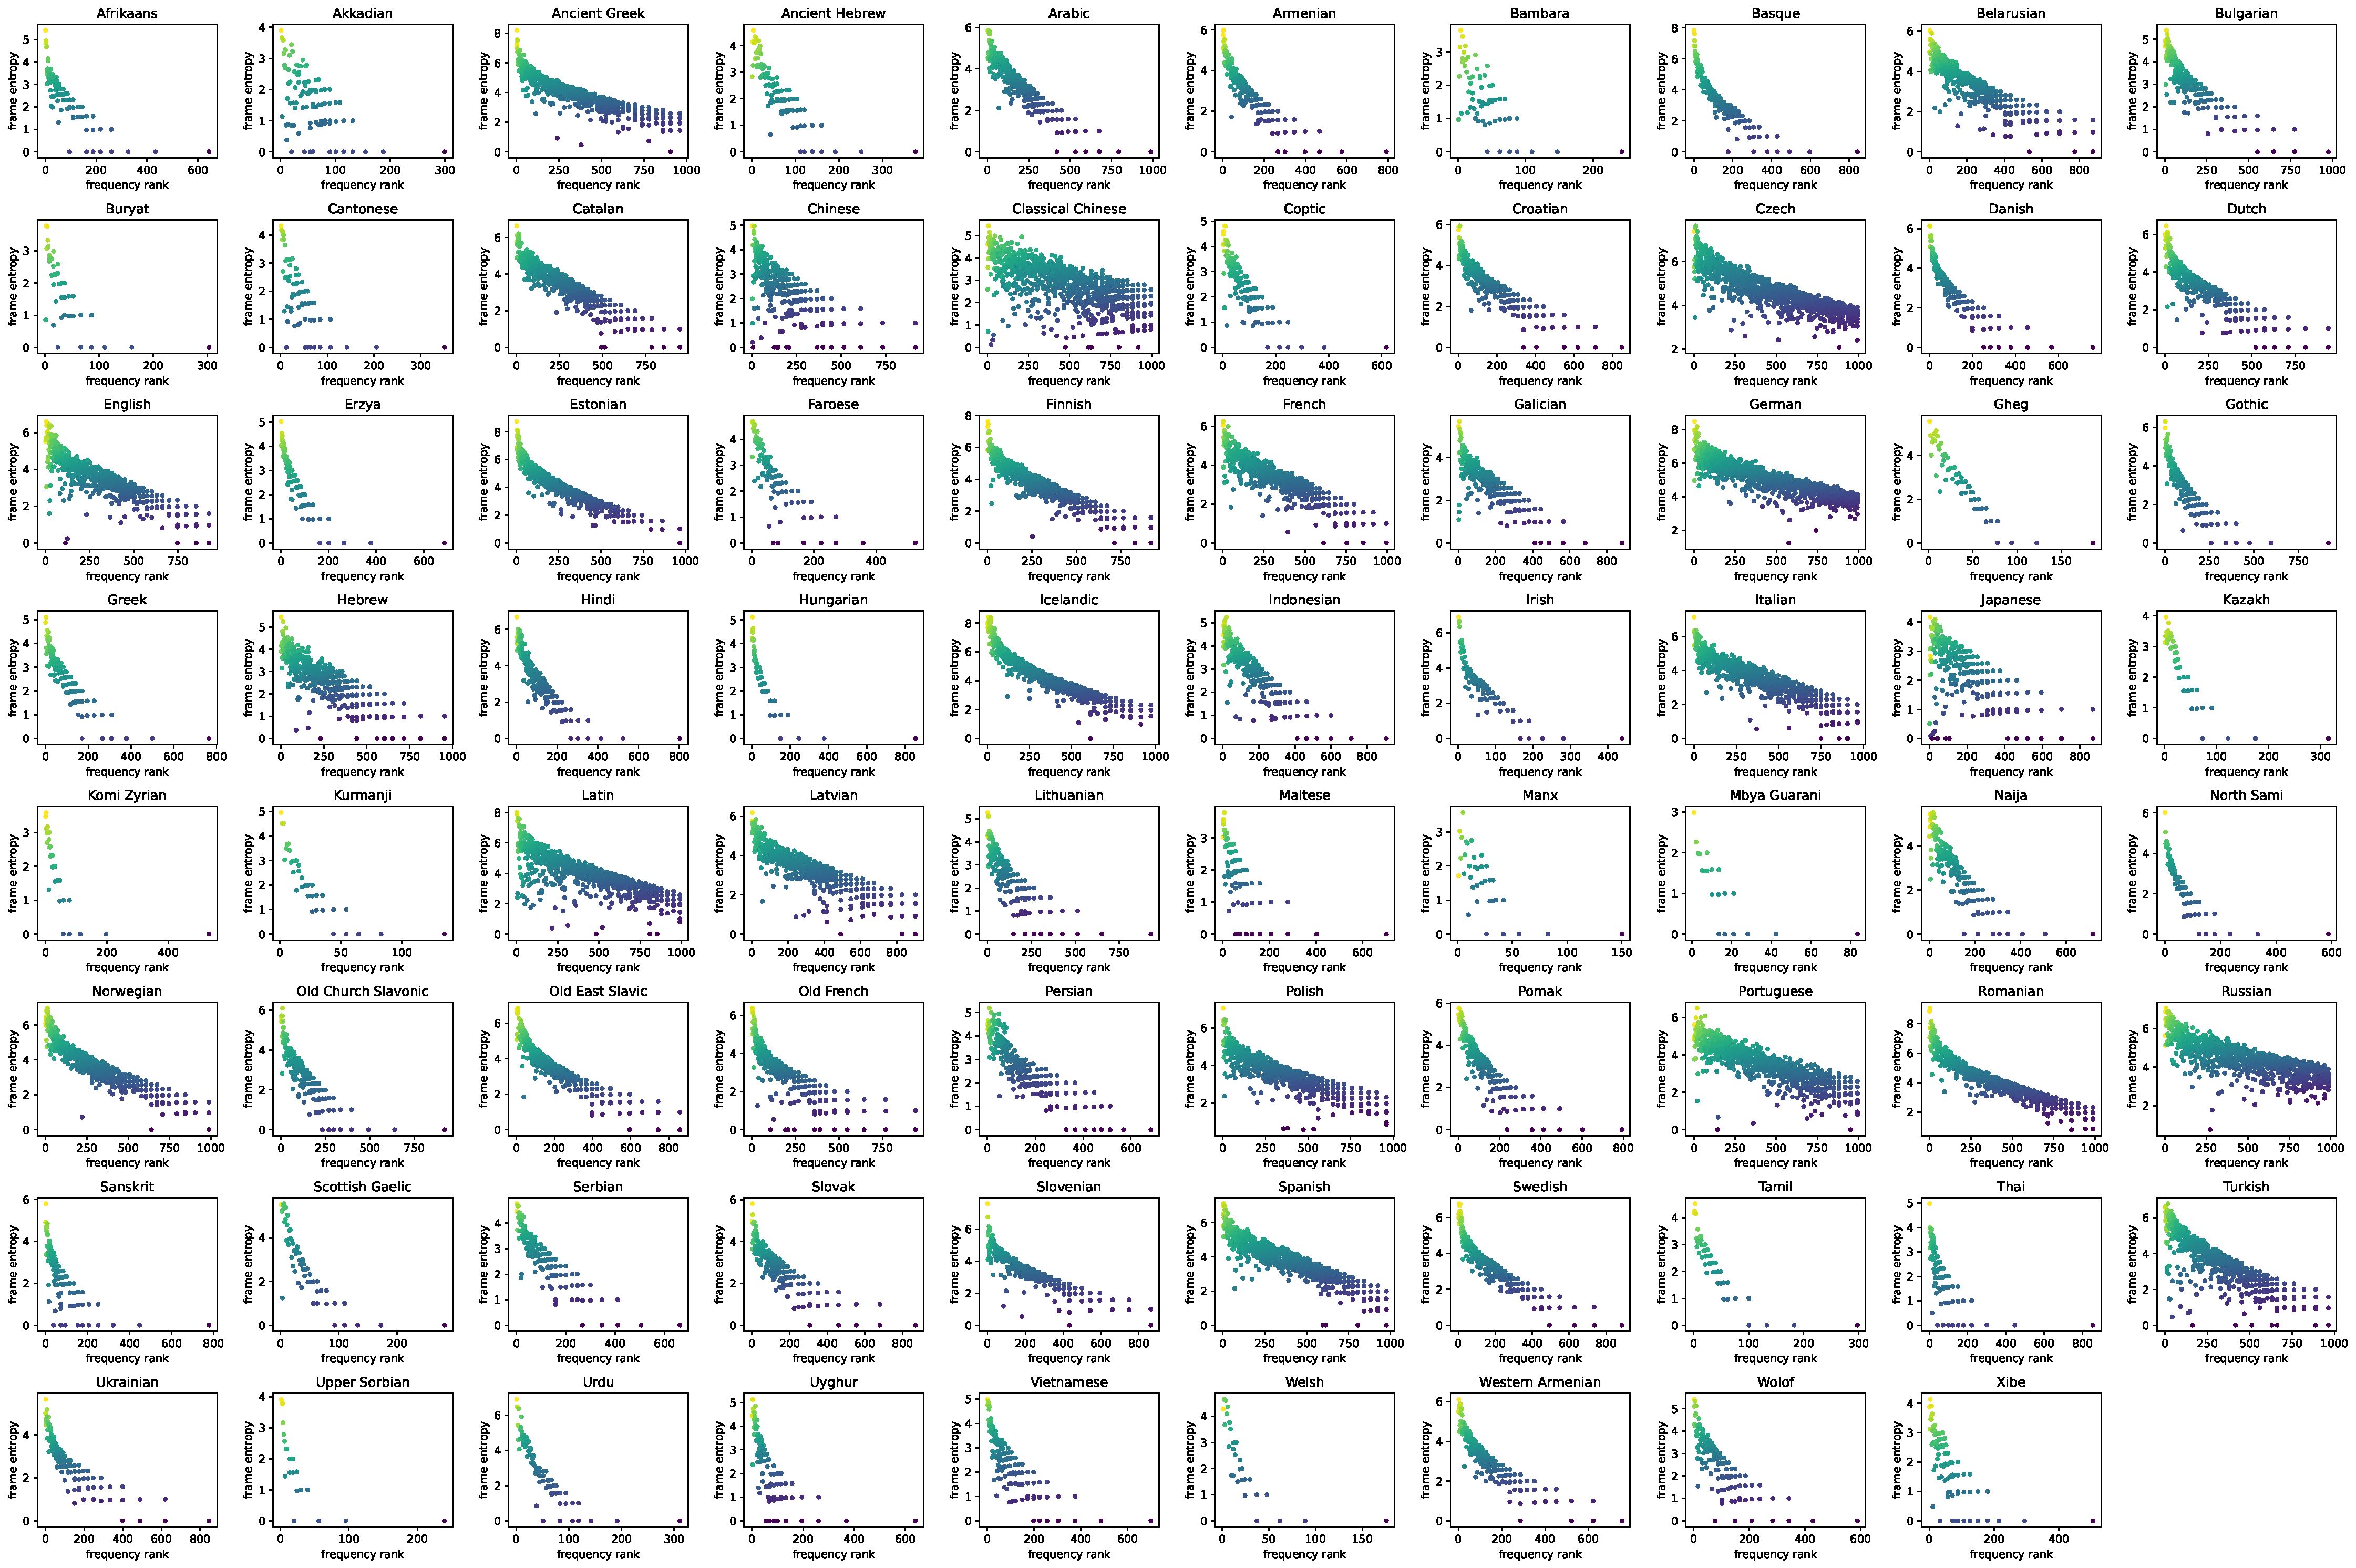
\includegraphics[width=\textwidth]{figures/joint_entropy_freq.pdf}
  \caption{Scatter plots showing relationship between valency frame entropy and frequency rank of verbs, color shows number of frames associated with the verb}
  \label{fig:joint_entropy_freq}
\end{sidewaysfigure}

\section{Experiment 3: Word order and case information}

\section{Experiment 4: Verb entropy}

\section{Experiment 5: Verb-finalness}
